\documentclass[11pt]{article}
\usepackage[utf8]{inputenc}
\usepackage[T1]{fontenc}
\usepackage{amsmath}
\usepackage{amssymb}
\usepackage{graphicx}
\usepackage{geometry}
\usepackage{booktabs} % For tables
\usepackage{tikz}
\usepackage{pgfplots} % For plots
\pgfplotsset{compat=1.17} % Enable axis cs: syntax
\usepackage{ulem}     % For underline, using normalem to avoid messing with \emph

\geometry{a4paper, margin=1in}
\usetikzlibrary{positioning, shapes.misc} % For TikZ diagrams
\pgfplotsset{compat=1.18} % Use a recent PGFPlots version

% Custom commands (optional)
\newcommand{\ddt}[1]{\frac{d #1}{dt}}
\newcommand{\dddt}[1]{\frac{d^2 #1}{dt^2}}
\newcommand{\avg}[1]{\overline{#1}}
\newcommand{\prob}[1]{P(#1)}
\newcommand{\vect}[1]{\vec{#1}}

\title{Physics 415 - Lecture 1: Statistical Mechanics (Preview)}
\date{January 22, 2025}
\author{} % Author not specified

\begin{document}

\maketitle
\thispagestyle{empty}

In statistical mechanics, we will be interested in the laws governing the behavior of "macroscopic" systems.
\begin{itemize}
    \item Macroscopic = composed of many constituent particles (atoms, molecules, etc.)
    \item Typical \# $\sim 10^{23}$ particles. % NOTE: Source says 1028, interpreting as 10^23
\end{itemize}
In principle, if "microscopic" (M-scopic) laws are known, then properties of systems of a large \# of particles can be deduced by solving the M-scopic equations.

\textbf{Example:} Classical system of N particles:
\[ m_i \ddot{\vec{r}}_i = \vec{F}_i(\vec{r}_1, \dots, \vec{r}_N), \quad i=1, \dots, N \]
(where $\dot{} \equiv \frac{d}{dt}$, $\ddot{} \equiv \frac{d^2}{dt^2}$, etc.)
Given initial conditions $\vec{r}_i(t=0)$ and $\vec{v}_i(t=0)$ ($\vec{v}_i = \dot{\vec{r}}_i$), we have complete knowledge of the state of the system at any time $t$.

However, for macroscopic N ($N \sim 10^{23}$), this is not feasible.
\begin{itemize}
    \item Even if we could solve the equations of motion (EOM), simply recording all initial conditions is not practical.
    \item Indeed, knowing the state of each particle is not even useful or interesting info.
    \item When the \# of particles is large, we'd rather have info about the "average" properties of the system.
\end{itemize}

Thus, in statistical mechanics, we will abandon such M-scopic determinism in favor of a statistical (or probabilistic) description.

We will find that, precisely because of the large \# of particles involved, new laws \& types of regularities will appear that govern the macroscopic behavior.
\begin{itemize}
    \item Notions like "entropy" \& "temperature" will emerge, that have no analog in particle mechanics \& are purely of statistical nature.
\end{itemize}

Since statistical notions will be important for understanding macroscopic systems, we'll spend some time reviewing basics of probability. This will be mostly math (not physics). We'll illustrate important ideas through an important example:

\section*{1D Random Walk}
(A good starting point for understanding a variety of phenomena).

\begin{center}
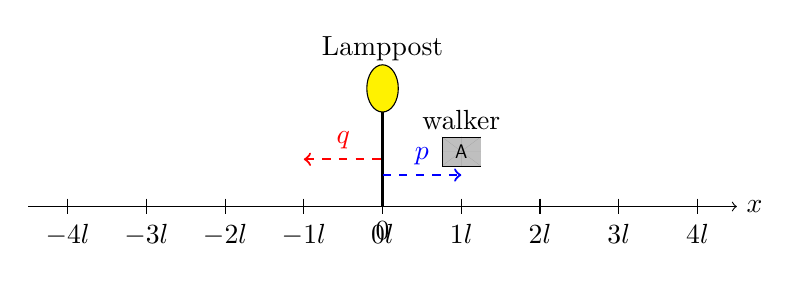
\begin{tikzpicture}
    % Axis
    \draw [->] (-4.5,0) -- (4.5,0) node [right] {$x$};
    \foreach \x/\label in {-4,...,4}{
        \draw (\x*1, 0.1) -- (\x*1, -0.1) node [below] {$\label l$};
    }
    \node at (0, -0.3) {0};

    % Lamppost
    \draw [thick] (0,0) -- (0,1.5);
    \draw [fill=yellow] (0,1.5) ellipse (0.2 and 0.3);
    \node at (0, 2) {Lamppost};

    % Walker
    \node[inner sep=0pt] (walker) at (1, 0.7) {\includegraphics[width=0.5cm]{example-image-a}}; % Placeholder for walker icon
    % \node[draw, circle, minimum size=0.5cm] (walker) at (1,0.4) {옷}; % Alternative text walker
    \node at (1, 1.1) {walker};

    % Steps description (optional)
    \draw [->, thick, dashed, blue] (0,0.4) -- (1*1, 0.4) node[midway, above] {$p$};
    \draw [<-, thick, dashed, red] (-1*1, 0.6) -- (0, 0.6) node[midway, above] {$q$};
\end{tikzpicture}
\end{center}

\begin{itemize}
    \item Walker starts from lamppost at $x=0$.
    \item Taking random steps of length $l$ at regular intervals.
    \item Each step is independent of the last.
    \item Probability $p$ to step to the right \& probability $q=1-p$ to step to the left.
\end{itemize}

\textbf{Question:} After taking $N$ steps, what is the probability that the walker is at a position $x=ml$ ($m=$ integer)?
(For another example of a 1D random walk, see "probability board" demo at Ingersoll museum).

We want to calculate the probability $P_N(m)$ that the walker is at position $x=ml$ after $N$ steps.
\begin{itemize}
    \item Let $n_1 = \#$ of steps right, $n_2 = \#$ of steps left.
    \item Total steps: $N = n_1 + n_2$.
    \item Final position: $ml = n_1 l - n_2 l \implies m = n_1 - n_2$.
    \item Note: $-N \le m \le N$. Also, $N$ and $m$ must have the same parity ($N-m = 2n_2$ is even).
    \item From the above, we can express $n_1$ and $n_2$ in terms of $N$ and $m$:
      $n_1 = (N+m)/2$
      $n_2 = (N-m)/2$
\end{itemize}

The probability of taking a specific sequence of $n_1$ steps right and $n_2$ steps left is:
\[ (\underbrace{p \times p \times \dots \times p}_{n_1 \text{ times}}) \times (\underbrace{q \times q \times \dots \times q}_{n_2 \text{ times}}) = p^{n_1} q^{n_2} \]
Of course, there are many different ways (sequences) in which the walker could take $n_1$ steps right \& $n_2$ steps left.

\textbf{Example:} $N=3$, $m=1$. Then $n_1=(3+1)/2=2$, $n_2=(3-1)/2=1$.
Possible sequences:
a) $\rightarrow \rightarrow \leftarrow$
b) $\rightarrow \leftarrow \rightarrow$
c) $\leftarrow \rightarrow \rightarrow$
There are 3 ways.

In general, the number of ways is given by the binomial coefficient:
\[ \text{\# of ways} = \binom{N}{n_1} = \frac{N!}{n_1! (N-n_1)!} = \frac{N!}{n_1! n_2!} \]
Check above example: $N=3, n_1=2, n_2=1 \implies \binom{3}{2} = \frac{3!}{2!1!} = 3$. $\checkmark$

Therefore, the total probability $P_N(m)$ is (number of ways) $\times$ (probability of one way):
\[ P_N(m) = \frac{N!}{n_1! n_2!} p^{n_1} q^{n_2} \]
This is the "binomial distribution".

Using $n_1 = (N+m)/2$ and $n_2 = (N-m)/2$:
\[ P_N(m) = \frac{N!}{[(N+m)/2]! [(N-m)/2]!} p^{(N+m)/2} (1-p)^{(N-m)/2} \]
Recall the binomial theorem: $(p+q)^N = \sum_{n_1=0}^{N} \frac{N!}{n_1!(N-n_1)!} p^{n_1} q^{N-n_1}$. Comparing with the formula for $P_N(m)$ (summed over $n_1$ or $m$) explains the name.

\textbf{Example:} $p=q=1/2$ (unbiased walk).
\[ P_N(n_1) = \frac{N!}{n_1! n_2!} \left(\frac{1}{2}\right)^N \]
Let's consider $N=10$. The probability $P_{10}(n_1)$ is plotted below.
Note: $m = n_1 - n_2 = n_1 - (N-n_1) = 2n_1 - N$.


% Table from source (approximations) - mapping index to n1 or m is slightly ambiguous in source
% Assuming index 0..5 corresponds to n1=0..5 based on values
\begin{center}
\begin{tabular}{cc}
\toprule
$n_1$ & Approx $P_{10}(n_1)$ \\
\midrule
0 & $\approx 0.001$ \\
1 & $\approx 0.01$ \\
2 & $\approx 0.044$ \\
3 & $\approx 0.12$ \\
4 & $\approx 0.21$ \\
5 & $\approx 0.25$ \\
\bottomrule
\end{tabular}
\end{center}

After $N=10$ steps, probability is largest for the particle to be near the origin ($m=0$, or $n_1=5$). Probability to be far from the origin is small.

\section*{General Notions}

Let $X$ be a random variable, taking $K$ possible values $x_1, x_2, \dots, x_K$, with associated probabilities $P(x_1), P(x_2), \dots, P(x_K)$.
($0 \le P(x_i) \le 1$ and $\sum_{i=1}^{K} P(x_i) = 1$).

\subsection*{Mean}
The "mean" (average) of $X$ is: $\avg{X} = \sum_{i=1}^{K} P(x_i) x_i$.
For a function $f(X)$: $\avg{f(X)} = \sum_{i=1}^{K} P(x_i) f(x_i)$.

\subsection*{Variance}
Suppose we want to know how much measurements of $X$ "fluctuate" about the mean value.
The "variance" (second moment, dispersion) is defined as:
% NOTE: Source had a typo (subscript 1), interpreting as standard definition
\[ \text{Var}(X) = \sigma_X^2 = \avg{(X - \avg{X})^2} = \sum_{i=1}^{K} P(x_i) (x_i - \avg{X})^2 \]
We square the deviation $(x_i - \avg{X})$ since fluctuations can have either sign.
Note the useful identity:
\[ \avg{(X - \avg{X})^2} = \avg{X^2 - 2X\avg{X} + (\avg{X})^2} = \avg{X^2} - 2\avg{X}\avg{X} + (\avg{X})^2 = \avg{X^2} - (\avg{X})^2 \]
We also define the root-mean-square (RMS) deviation (or standard deviation):
% NOTE: Corrected typo in source formula for RMS
\[ \Delta X_{rms} = \sigma_X = \sqrt{\avg{(X - \avg{X})^2}} = \sqrt{\avg{X^2} - (\avg{X})^2} \]

\textbf{Example:} Binomial Distribution Properties (results to be shown in discussion section/homework)
\begin{itemize}
    \item Average \# of steps to the right: $\avg{n_1} = N \times p$ \\
    ($= (\text{total \# of steps}) \times (\text{prob. of step right})$)
    \item Variance: $\text{Var}(n_1) = \avg{n_1^2} - (\avg{n_1})^2 = N \times p q$
    \item RMS deviation: $\Delta n_{1, rms} = \sqrt{N p q}$
    \item The relative width is:
    \[ \frac{\Delta n_{1, rms}}{\avg{n_1}} = \frac{\sqrt{Npq}}{Np} = \sqrt{\frac{q}{p}} \times \frac{1}{\sqrt{N}} \]
    \item This shows the distribution becomes sharply peaked ($\text{relative width} \to 0$) when $N \gg 1$.
\end{itemize}

\end{document}